\documentclass{beamer}
\usepackage[utf8]{inputenc}
\usepackage[T1]{fontenc}
\usepackage{graphicx}
\usepackage{grffile}
\usepackage{longtable}
\usepackage{wrapfig}
\usepackage{rotating}
\usepackage[normalem]{ulem}
\usepackage{amsmath}
\usepackage{textcomp}
\usepackage{amssymb}
\usepackage{capt-of}
\usepackage{hyperref}
\newcommand{\inlinelatex}[1]{#1}
\usetheme{Madrid}
\setbeamertemplate{frametitle continuation} {}
\title[CMP223]{Performance and Cost-Aware in HPC: A Network Interconnect Impact Assessment}
\author[Anderson M.M]{\large{Anderson M. Maliszewski}}
\institute[UFRGS]{\small{Parallel and Distributed Processing Group (GPPD)\\
Informatics Institute (INF)\\
Federal University of Rio Grande do Sul (UFRGS) \\Porto Alegre - Brazil}}
\date[11 December, 2019]{\large{CMP223 Computer System Performance Analysis (2019/2)\\
11 December, 2019}}
\logo{
\includegraphics[width=1.3cm,keepaspectratio]{SLIDES/logo/ufrgs.png}~~~~~~~~~~~~~~~~~~~~~~~~~~~~~~~~~~~~~~~~~~~~~~~~~~~~~~~~~~~~~~~~~~~~~
%\hspace{\dimexpr\paperwidth-5cm-1pt}%
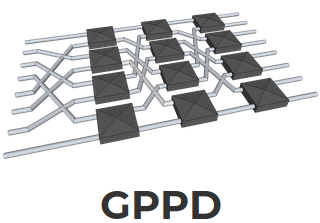
\includegraphics[width=1.3cm,keepaspectratio]{SLIDES/logo/GPPD-logo.png}~~~~~~~~~~~~~~~~~~~~~~~~~~~~~~~~~~~~~~~~~~~~~~~~~~~~~~~~~~~~~~~~~~~~~
%\hspace{\dimexpr\paperwidth-3cm-1pt}%

\includegraphics[width=1.5cm,keepaspectratio]{SLIDES/logo/inf-logo.png}%
}

\colorlet{beamer@blendedblue}{black}
\setbeamercolor{alerted text}{fg=orange}

\begin{document}
\maketitle
\logo{
\includegraphics[width=1.5cm]{SLIDES/logo/inf-logo.png}}
\begin{frame}{Introduction}
\vfill
Growing demand for \alert{computational power}
\begin{itemize}
\item High Performance Computing (HPC)
\item Clusters and "as a Service" cloud models
\end{itemize}
\pause \vfill
\alert{Communication characteristics} vary from application to application
\begin{itemize}
\item Application specific proposal
\item Bandwidth and latency-sensitive
\end{itemize}
\pause \vfill
Network interconnection is directly related to \alert{performance losses}
\begin{itemize}
\item High performance interconnects - InfiniBand
\end{itemize}
\end{frame}

\begin{frame}{Motivation}
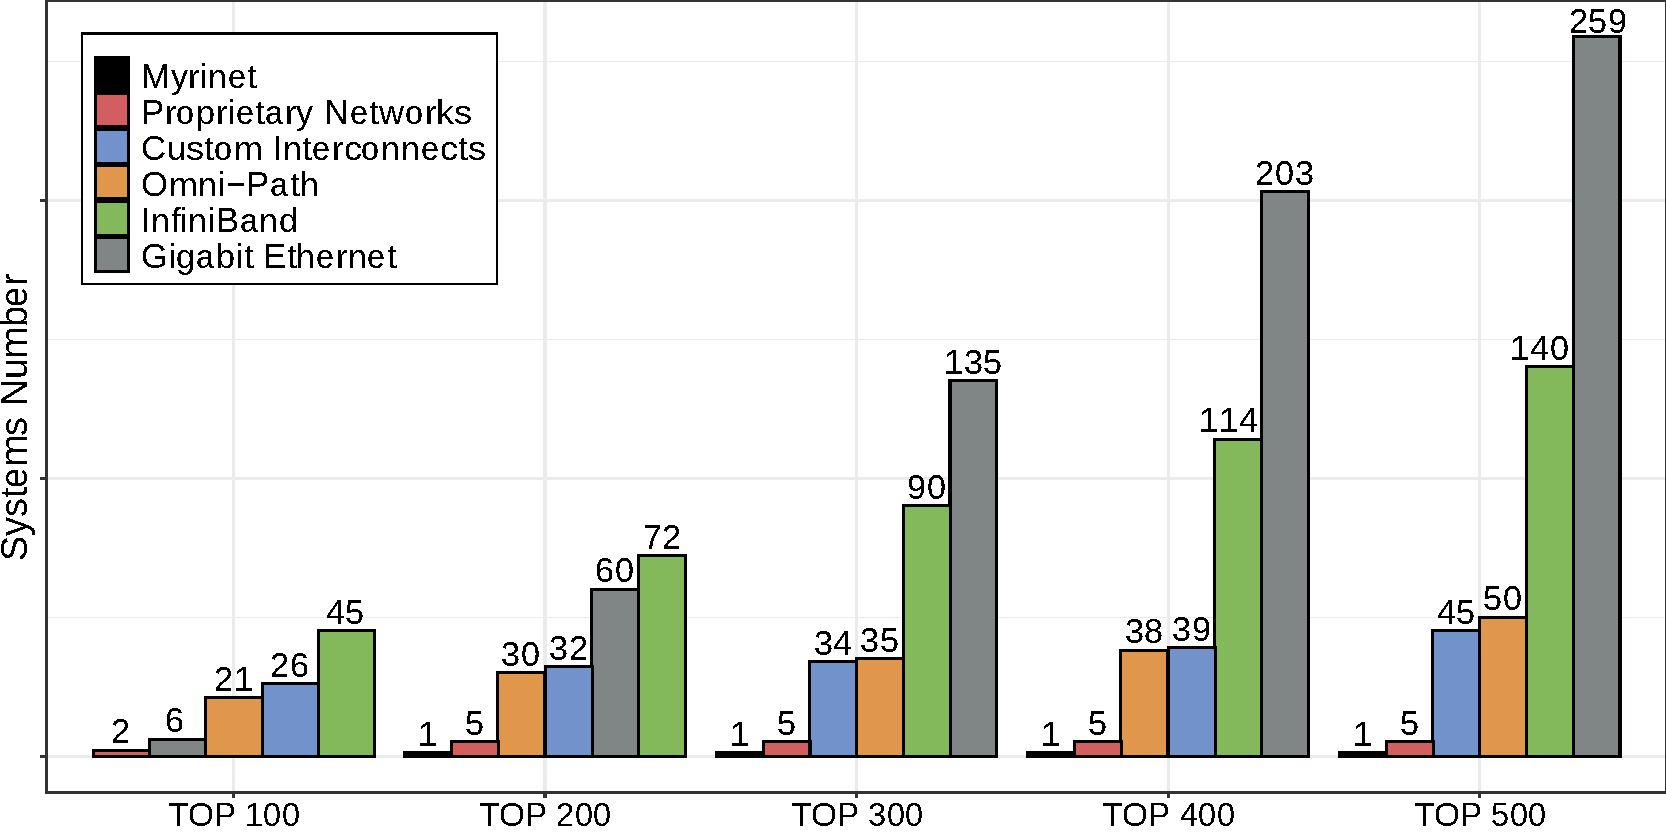
\includegraphics[width=\textwidth]{SLIDES/img/TOP500-5.pdf}
\end{frame}

\begin{frame}{Problem Statement}
How do the \alert{communication characteristics} of applications influence their \alert{performance}?
\pause \vfill
Is it possible to optimize both \alert{performance} and \alert{execution cost} just by using another interconnect?
\pause \vfill
To answer these questions:

\pause \vfill
\begin{itemize}
    \item Both 1 Gbps Ethernet (ETH) and InfiniBand FDR 56 Gbps (IB) interconnects were evaluated using the same physical server cluster, using applications with different requests
\pause \vfill
    \item All applications were also traced, exposing their communication and computing characteristics both rank by rank and as a percentage
\pause \vfill
    \item Finally, the execution cost was calculated using the Microsoft Azure instance pricing model, where the instances in question \\(A8 and A10) have the same hardware, differing only by the interconnect used (IB and Ethernet)
\end{itemize}
\vfill
    
\end{frame}
\begin{frame}{Outline}
\vfill
\Large
\begin{itemize}
\item Methodology
\begin{itemize}
\item System
\item Testbed
\item Applications
\item Tracing Process
\item Experimental Design
\item Reproducible Research Methodology
\end{itemize}
\end{itemize}
\begin{itemize}
\item Results
\begin{itemize}
    \item Latency
    \item Bandwidth
    \item Execution time
    \item Execution cost
    \item Characterization
\end{itemize}
\end{itemize}
\begin{itemize}
\item Conclusion
\item Future Work
\end{itemize}
\end{frame}

\begin{frame}  [plain, noframenumbering]
\begin{block}{}
\begin{center}
\Huge{Methodology}
\end{center}
\end{block}
\end{frame}

\begin{frame}[noframenumbering, allowframebreaks]{System}
\vspace{-0.7cm}
\begin{center}
    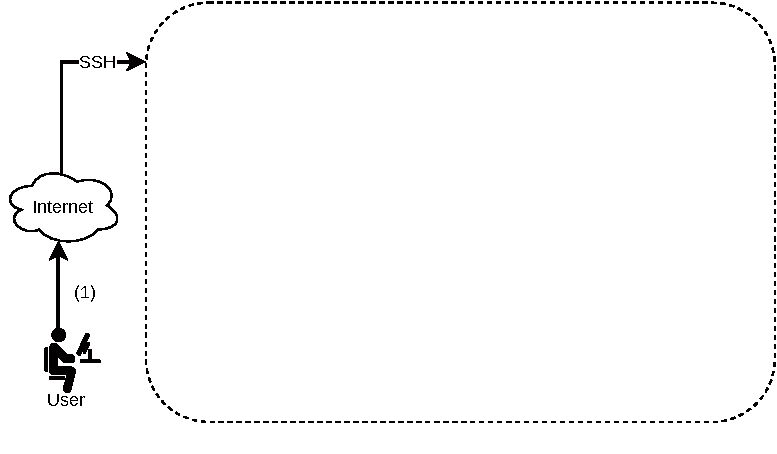
\includegraphics[scale=0.65]{SLIDES/img/System1.pdf}
\end{center}
    \begin{itemize}
    \item (1) The user submits a job through the Internet using SSH in this case
    \item[~] 
    \item[~]
    \item[~] 
    \end{itemize}
    \framebreak
\begin{center}
    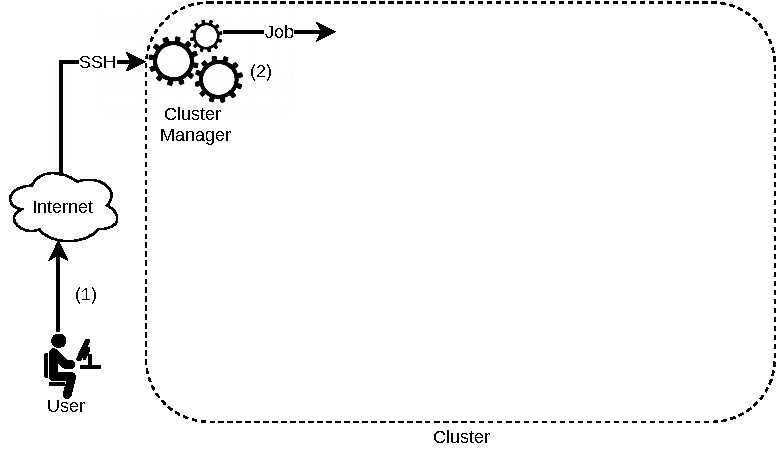
\includegraphics[scale=0.65]{SLIDES/img/System2.pdf}
\end{center}
    \begin{itemize}
    \item (1) The user submits a job through the Internet using SSH in this case
    \item (2) Cluster manager allocates nodes using its own policy based for example on node availability
    \item[~] 
    \item[~]
    \end{itemize}
    \framebreak
\begin{center}
    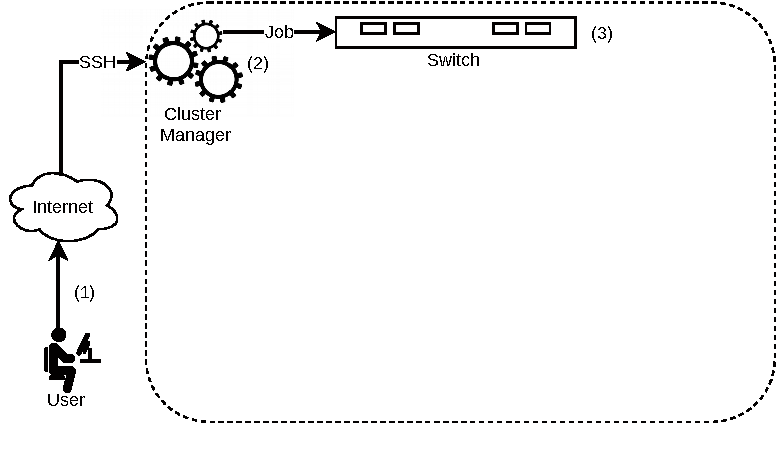
\includegraphics[scale=0.65]{SLIDES/img/System3.pdf}
\end{center}    
    \begin{itemize}
    \item (1) The user submits a job through the Internet using SSH in this case
    \item (2) Cluster manager allocates nodes using its own policy based for example on node availability
    \item (3) Job is passed to nodes via a switch
    \item[~]
    \end{itemize}
    \framebreak
\begin{center}
    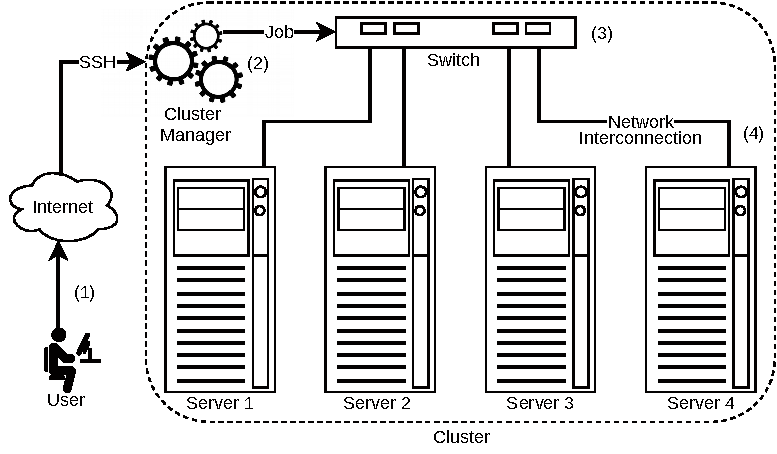
\includegraphics[scale=0.65]{SLIDES/img/System4.pdf}
\end{center}    
    \begin{itemize}
    \item (1) The user submits a job through the Internet using SSH in this case
    \item (2) Cluster manager allocates nodes using its own policy based for example on node availability
    \item (3) Job is passed to nodes via a switch
    \item (4) The switch acts as a central point of nodes communication
    \end{itemize}
\end{frame}

\begin{frame}{Testbed}
PCAD's Hype cluster \footnote{[1] http://gppd-hpc.inf.ufrgs.br/}
\begin{itemize}
\item 2 \texttimes{} Intel Xeon E5-2650 v3 (Q3'14) Haswell, 2.3 GHz
\item 20 cores (10 per CPU) with HT enabled resulting in 40 threads
\item 128 GB DDR4 RAM
\item Gigabit Ethernet and InfiniBand FDR interconnects
\item Ubuntu Server 18.04.01
\end{itemize}
\end{frame}

\begin{frame}{Applications}
Network characterization (Bandwidth and Latency)
    \begin{itemize}
        \item Intel MPI Benchmarks 
        \begin{itemize}
            \item PingPong
        \end{itemize}
    \end{itemize}
    \pause \vfill
Synthetic applications performance
    \begin{itemize}
        \item NPB 3.4 MPI
        \begin{itemize}
            \item BT, CG, EP, FT, IS, LU, MG, and SP
            \item Input class D
        \pause \vfill
        \end{itemize}
        \item ImbBench 
        \begin{itemize}
            \item CPU and Memory
            \item 8 Levels of Imbalance
        \end{itemize}
        \end{itemize}
        \pause \vfill
Real application performance
    \begin{itemize}
        \item Alya
    \end{itemize}
\end{frame}

\begin{frame}{Tracing Process}
To trace the applications were used:
\pause \vfill
    \begin{itemize}
        \item Score-P Version 6.0
        \begin{itemize}
            \item Used to compile applications and thus make data collection possible
        \end{itemize}
    \pause \vfill
        \item Akypuera
        \begin{itemize}
            \item \texttt{otf22paje}
                \begin{itemize}
                    \item Convert the files
                \end{itemize}
        \end{itemize}
    \pause \vfill
        \item PajeNG
        \begin{itemize}
            \item \texttt{pj\_dump}
                \begin{itemize}
                    \item Convert files to a CSV for parsing them in R
                \end{itemize}
        \end{itemize}
    \end{itemize}
\end{frame}


\begin{frame}{Experimental Design}
It was created using the DoE.base library in R
\begin{itemize}
    \item Follows a full factorial design
    \item Two levels for each execution
 \begin{itemize}
\item Application: \alert{BT}, \alert{EP}, \alert{CG}, \alert{MG}, \alert{LU}, \alert{SP}, \alert{IS}, \alert{FT}, \alert{IMB\_Memory}, \alert{IMB\_CPU}, \alert{PinPong}, and \alert{Alya}
\item Network Interface: \alert{Gigabit Ethernet} and \alert{InfiniBand}
\end{itemize}
    \item 30 randomized replications
   \end{itemize}
N = (12 applications) \texttimes{} (2 interconnections) \texttimes{} (30 replications) = 720 experiments
\pause \begin{itemize}
    \item In the characterization execution the PingPong application was not executed and only one replication was performed, totaling in N = (11 applications) \texttimes{} (2 interconnections) = 22 experiments  

\end{itemize}
\end{frame}

\begin{frame}{Reproducible Research Methodology}
\vfill
A main execution script
\begin{itemize}
    \item No user interaction
    \item Collect system information
    \item Download all softwares/applications and compile them
    \item Execute and collect the results
\end{itemize}

\pause Org and Emacs
\begin{itemize}
    \item LabBook
    \item R Blocks of code
\end{itemize}

\pause GitHub
\begin{itemize}
    \item All scripts are public
    \item Description of files and folders with softwares used/needed to accurately reproduce this evaluation
    \item If something is wrong, anyone can open a ``Issue''
\end{itemize}

\pause Zenodo
\begin{itemize}
    \item As this work has logs that add up to 117G, these \\will be zipped and sent to Zenodo
\end{itemize}
\end{frame}


\begin{frame} [plain, noframenumbering]
\begin{block}{}
\begin{center}
\Huge{Results}
\end{center}
\end{block}
\end{frame}

\begin{frame}{Network Latency}
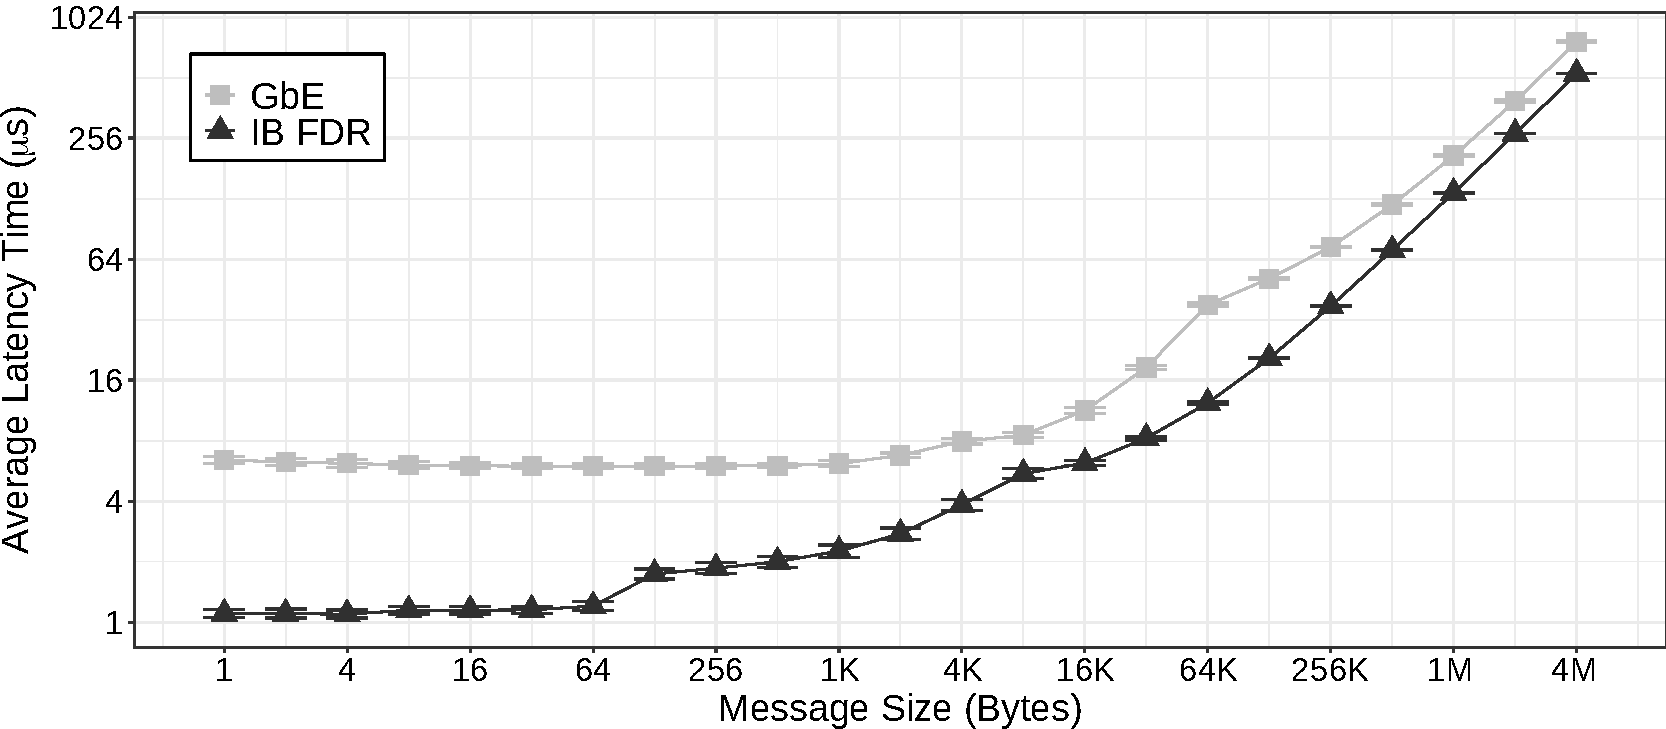
\includegraphics[width=\textwidth]{SLIDES/img/Latency.pdf}
\vfill\pause
\pause Observations
\begin{itemize}
    \item InfiniBand latency is much lower\\
        $\to$ Similar results observed in the literature
\end{itemize}
\end{frame}


\begin{frame}{Network Bandwidth}
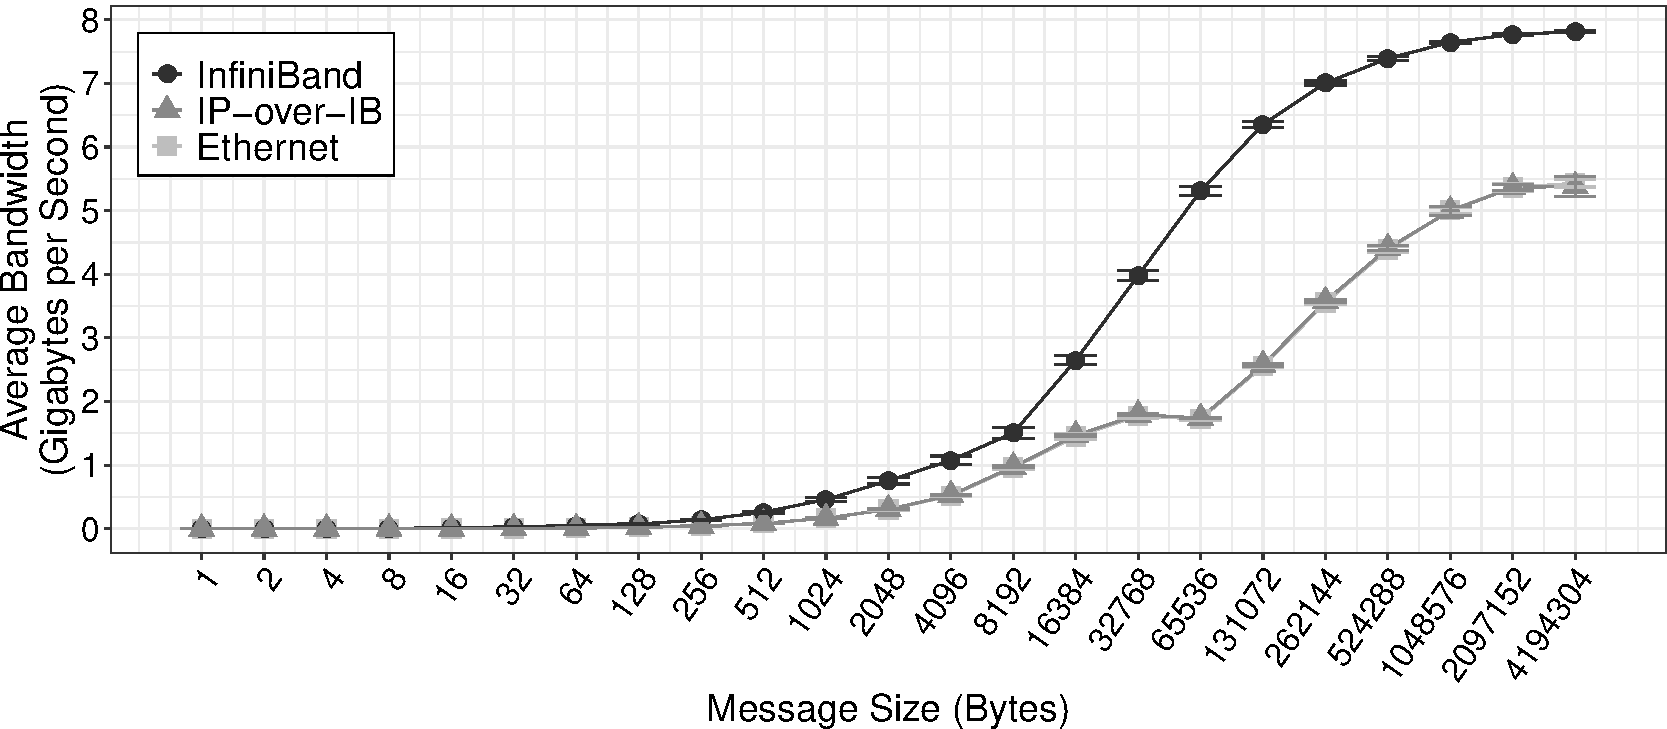
\includegraphics[width=\textwidth]{SLIDES/img/Bandwidth.pdf}
\vfill\pause
\pause Observations
\begin{itemize}
    \item InfiniBand's bandwidth begins to show a big difference \\(for better) from 1024 Bytes messages
\end{itemize}
\end{frame}

\begin{frame}{Analysis Of Interesting Cases (Execution Time)}
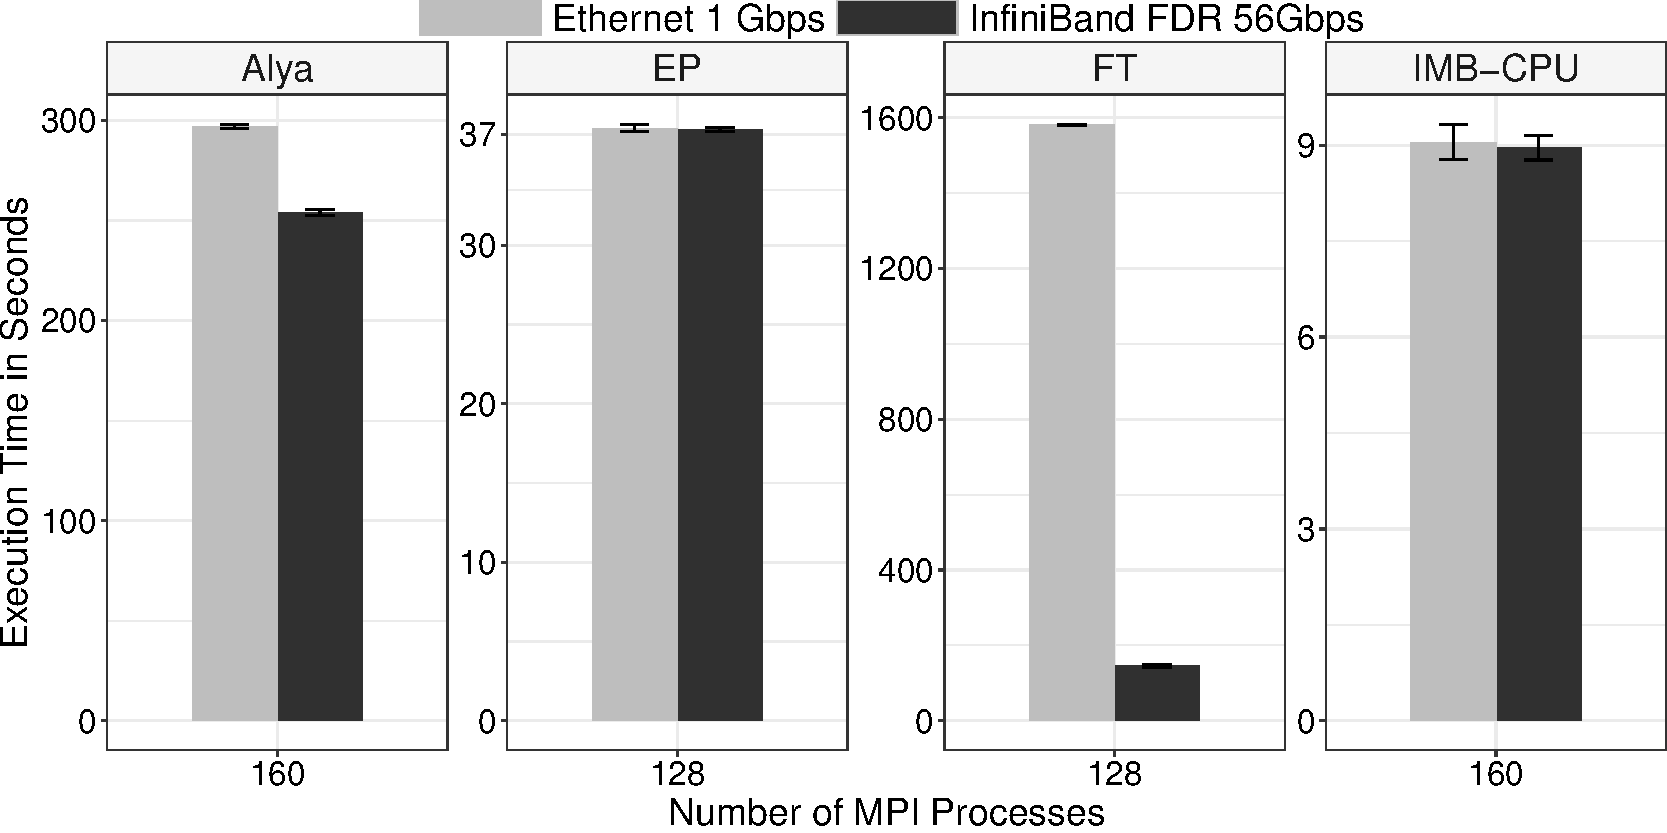
\includegraphics[width=\textwidth]{SLIDES/img/FT-EP-Alya-IMB.pdf}
Observations
\begin{itemize}
    \pause\item Alya performance is increased by up to $\approx$16\% using IB
    \pause\item EP and IMB performance for both ETH and IB overlaps
    \pause\item FT have a enormous gain using IB (up to $\approx$989\%)
\end{itemize}
\end{frame}

\begin{frame}{Analysis Of Interesting Cases (Execution Cost)}
\vspace{-0.5cm}
\begin{center}
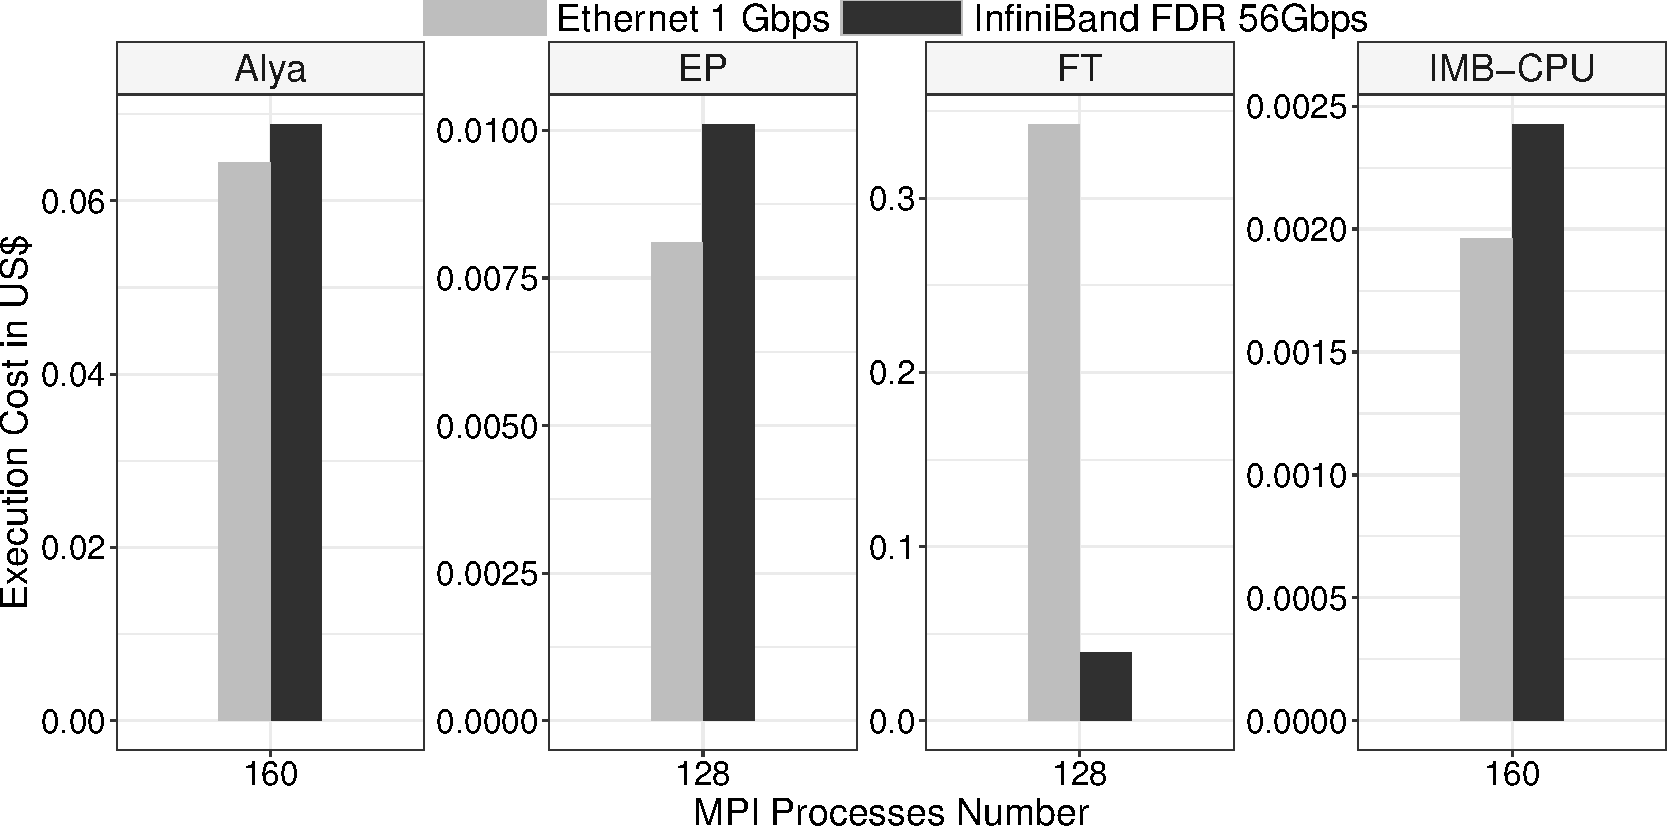
\includegraphics[scale=0.3]{SLIDES/img/FT-EP-Alya-IMB.cost.pdf}
\end{center}
\vspace{-0.5cm}
\begin{table}[h]
\resizebox{\textwidth}{!} \\
{\color[HTML]{000000} EP} & {\color[HTML]{000000} US\$ 0.03} & {\color[HTML]{000000} US\$ 0.04} & {\color[HTML]{000000} US\$ -0.01} & {\color[HTML]{000000} -19.81\%} \\
{\color[HTML]{000000} FT} & {\color[HTML]{000000} US\$ 1.36} & {\color[HTML]{000000} US\$ 0.16} & {\color[HTML]{000000} US\$ 1.21} & {\color[HTML]{000000} 770\%} \\
{\color[HTML]{000000} IMB-CPU} & {\color[HTML]{000000} US\$ 0.0078} & {\color[HTML]{000000} US\$ 0.0097} & {\color[HTML]{000000} US\$ -0.0019} & {\color[HTML]{000000} -19.59\%} \\ \hline
\end{tabular}%
}
\end{table}
\begin{itemize}
    \item A8 (IB) costs US\$ 0.975 and A10 (ETH) US\$ 0.78 per hour
\end{itemize}
\end{frame}

\begin{frame}{Analysis Of Interesting Cases (Characterization - Alya)}
\begin{figure}
   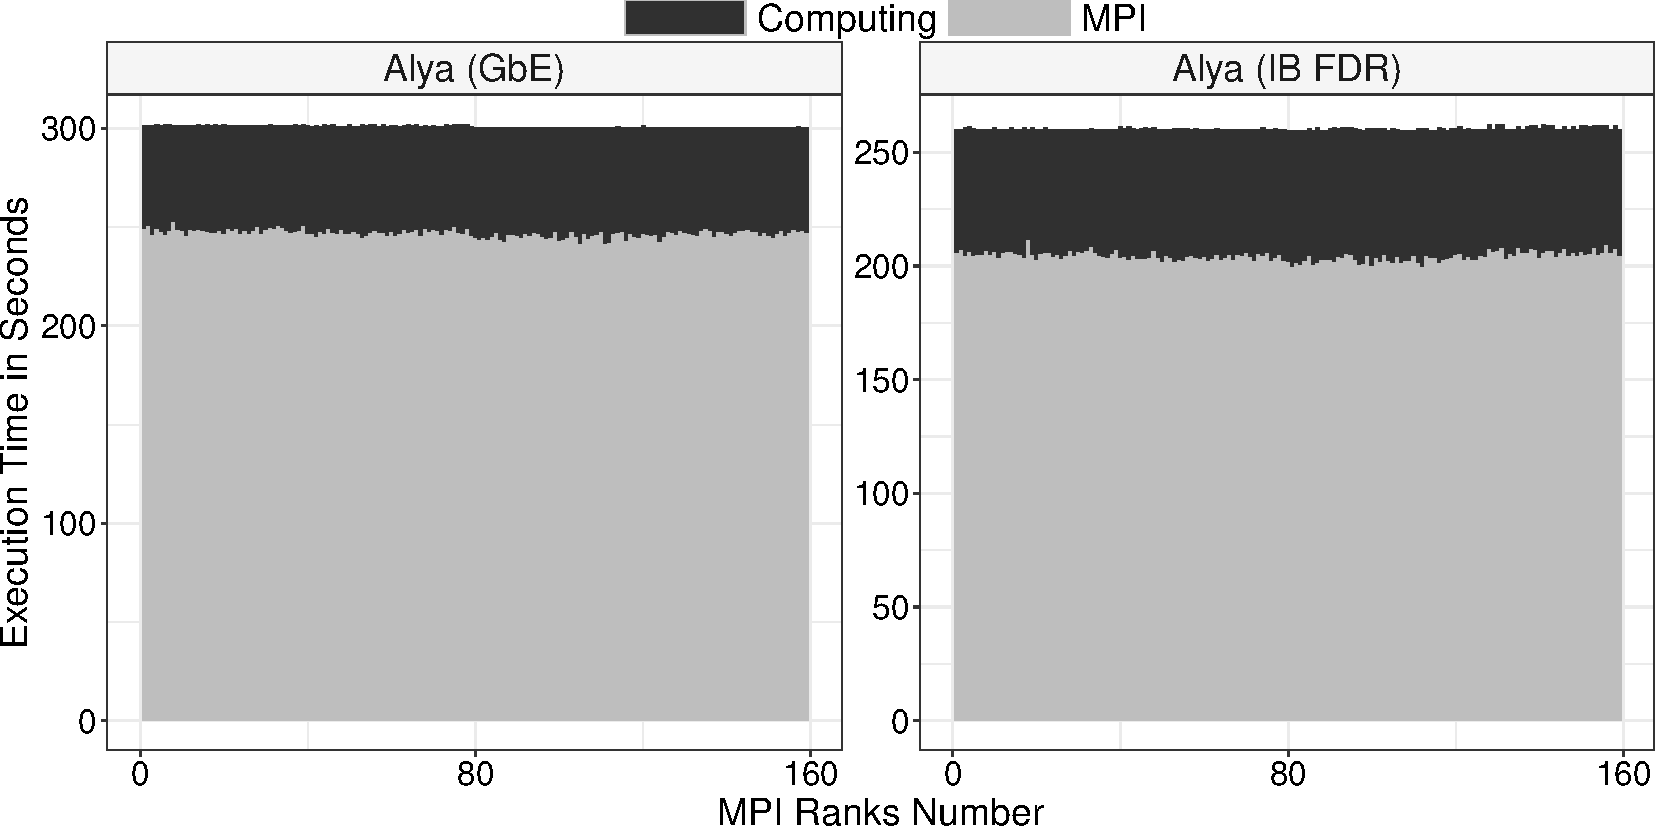
\includegraphics[width=0.61\textwidth]{SLIDES/img/Alya.charac.pdf}
   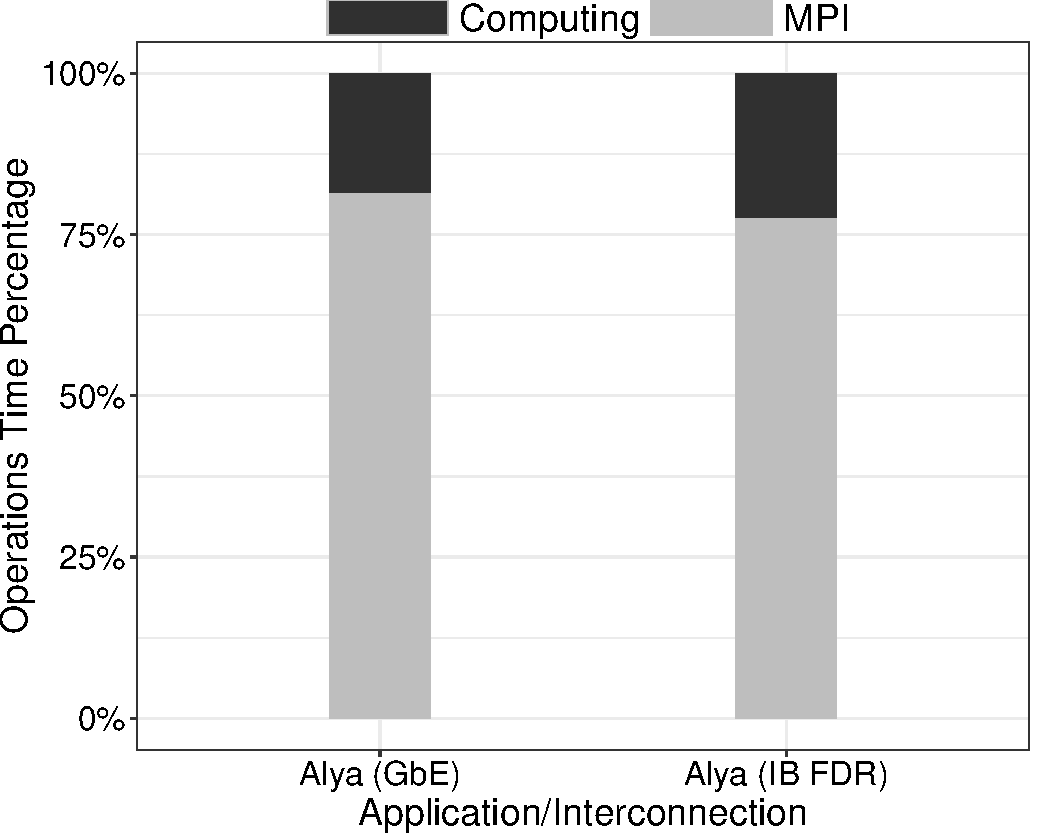
\includegraphics[width=0.38\textwidth]{SLIDES/img/Alya.percentage.pdf}
\end{figure}
Observations
\begin{itemize}
    \pause\item Based on the plot with MPI Ranks (left side), this app follows a straight line to be almost perfectly balanced
    \pause\item Both ETH and IB have almost the same pattern with different execution times
    \pause\item In the percentage graph (right side), the results show that both interconnections have almost the same computation and MPI percentage between them
\end{itemize}
\end{frame}

\begin{frame}{Analysis Of Interesting Cases (Characterization - EP)}
\begin{figure}
   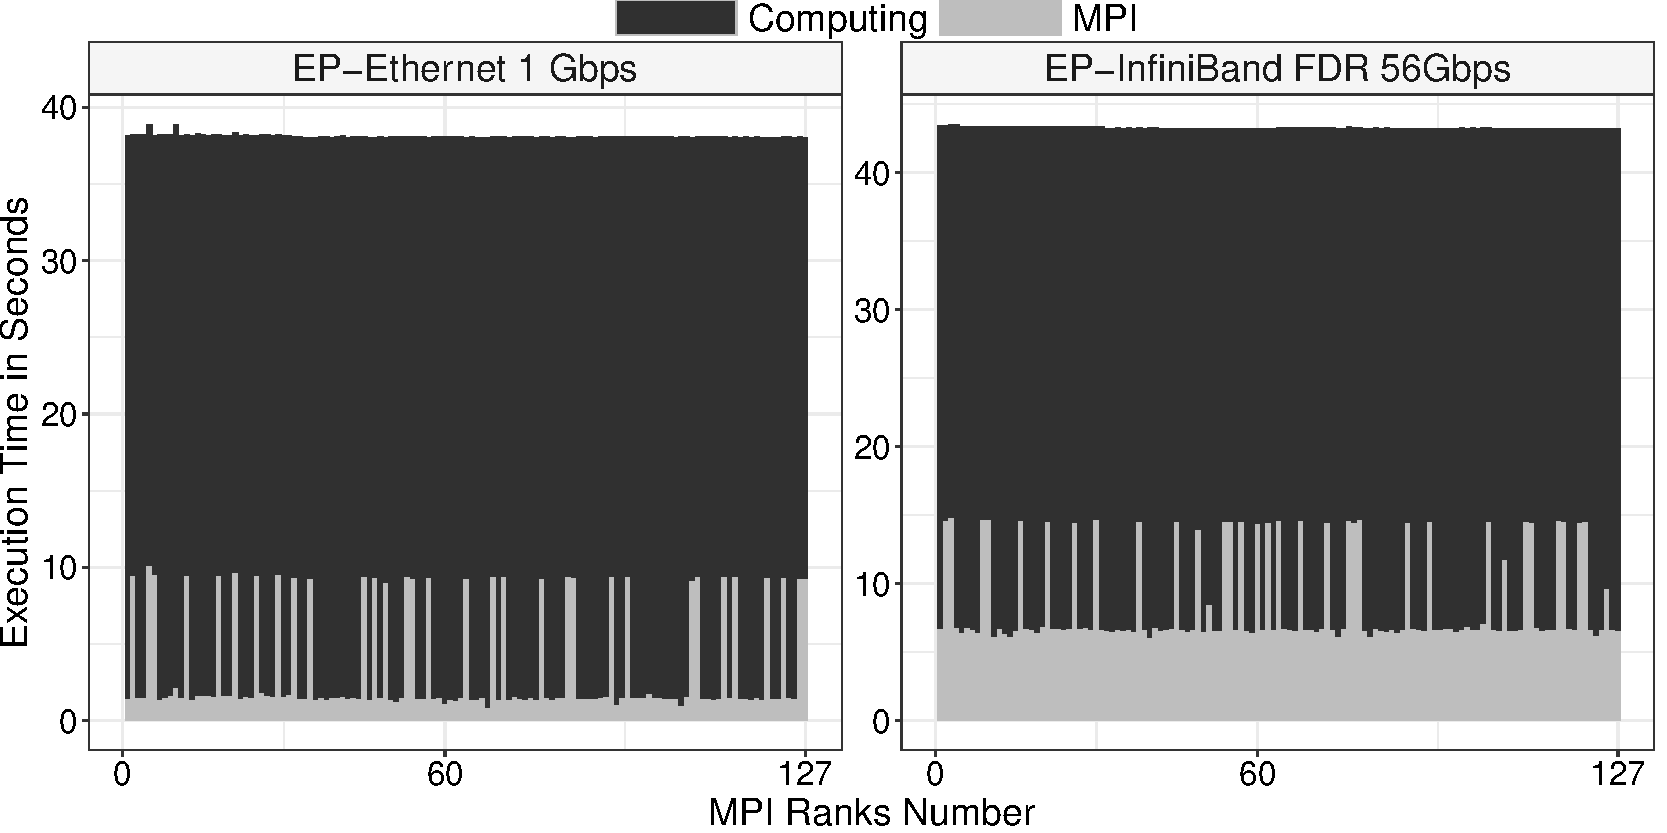
\includegraphics[width=0.61\textwidth]{SLIDES/img/EP.charac.pdf}
   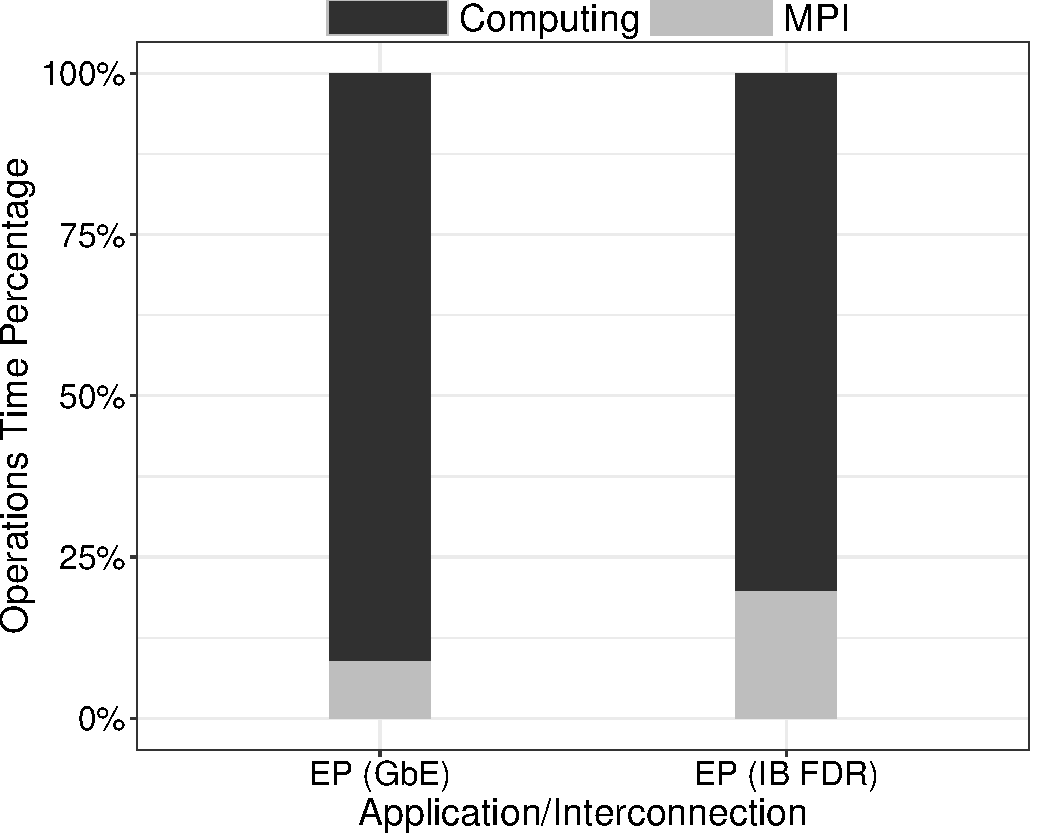
\includegraphics[width=0.38\textwidth]{SLIDES/img/EP.percentage.pdf}
\end{figure}
Observations
\begin{itemize}
    \pause\item This application is dominated by Computing, with some rankings having MPI spikes
    \pause\item In IB, the MPI\_Init operation has a longer execution time, which sets it apart from ETH
    \pause\item The total percentage of MPI and Computing confirms the \\above explanation, in which ETH has a bigger Computing \\and a smaller MPI than ETH   
\end{itemize}

\end{frame}

\begin{frame}{Analysis Of Interesting Cases (Characterization - FT)}
\begin{figure}
   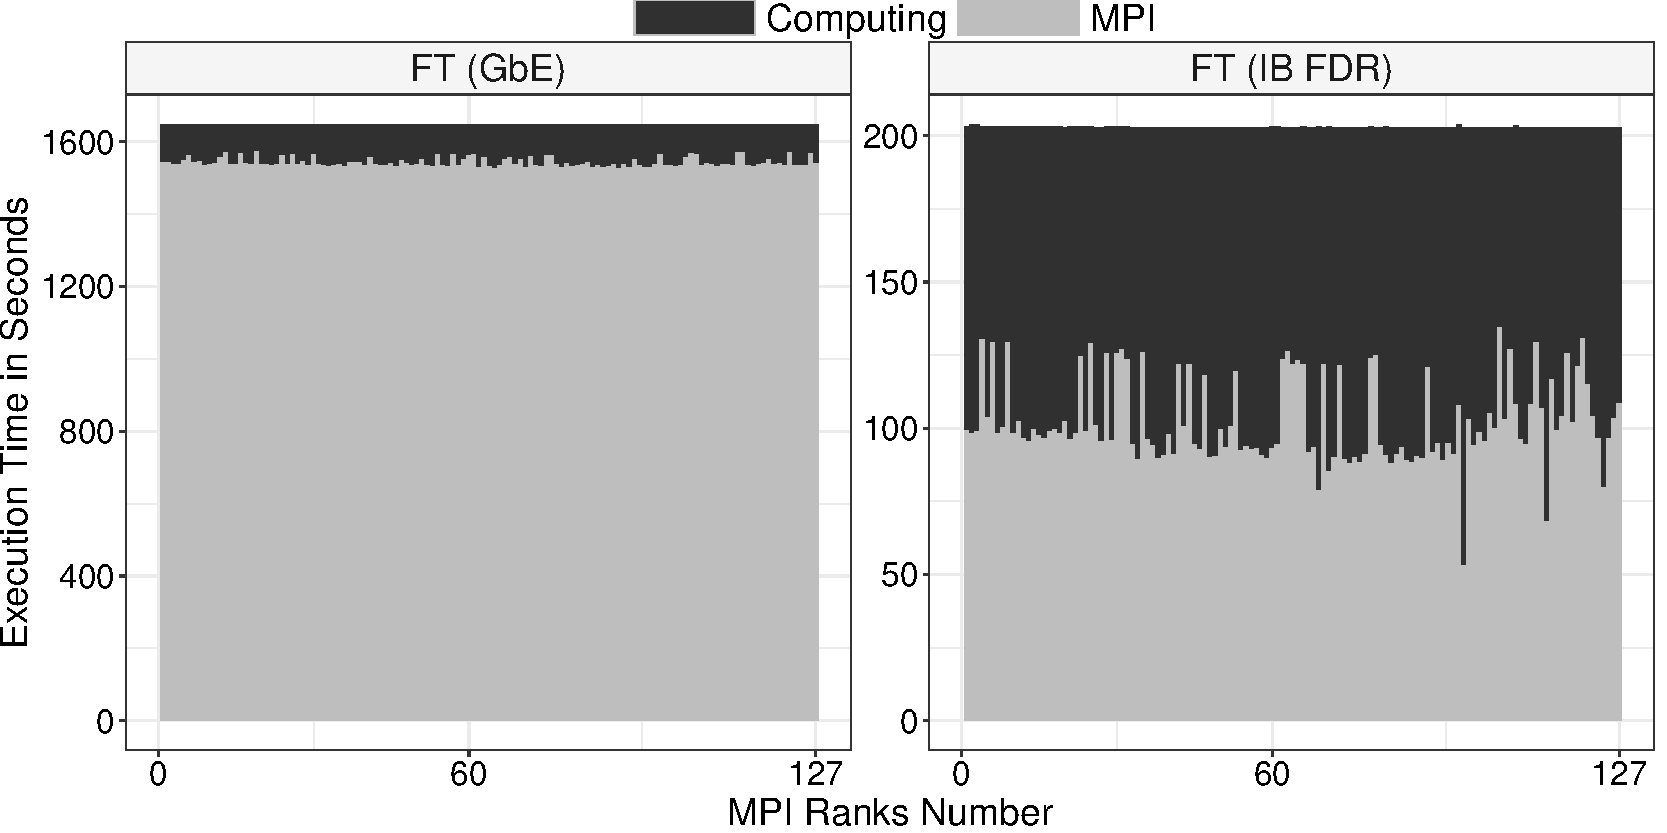
\includegraphics[width=0.61\textwidth]{SLIDES/img/FT.charac.pdf}
   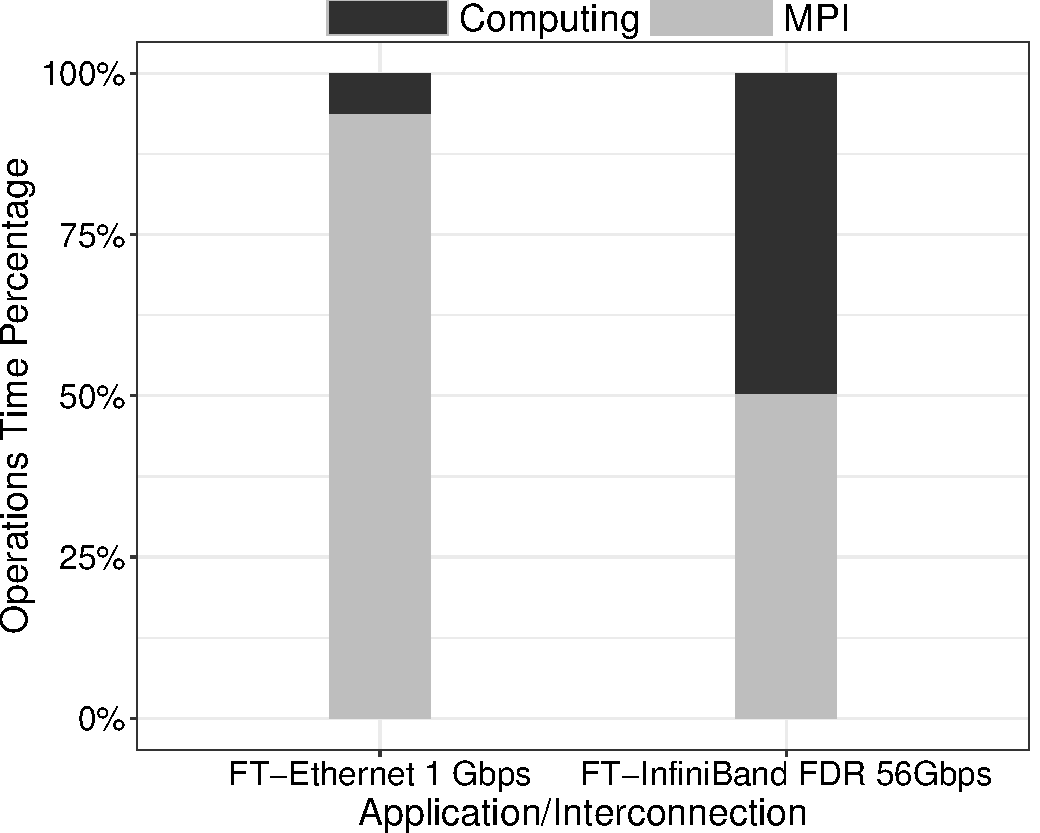
\includegraphics[width=0.38\textwidth]{SLIDES/img/FT.percentage.pdf}
\end{figure}
Observations
\begin{itemize}
    \pause \item FT has the pattern of sending several MPI messages, which makes it communication intensive
    \pause \item In ETH, it is dominated by MPI operations, therefore its time is high
    \pause \item On the other hand, in IB, both MPI and Computing \\operations reaches $\approx$50\%
\end{itemize}
\end{frame}

\begin{frame}{Analysis Of Interesting Cases (Characterization - IMB CPU)}
\begin{figure}
   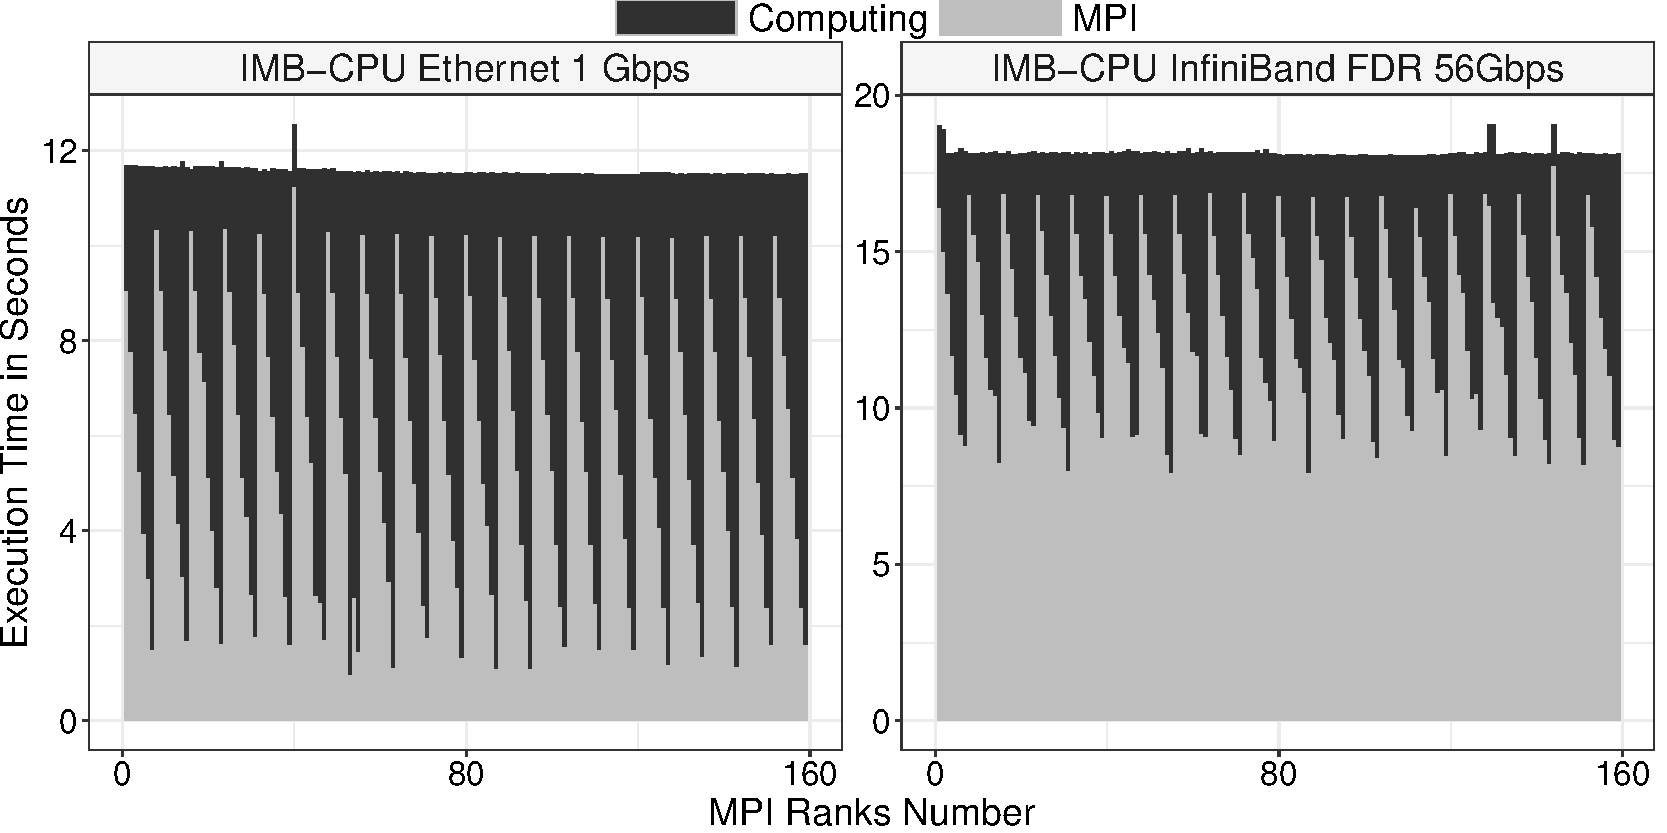
\includegraphics[width=0.61\textwidth]{SLIDES/img/IMB-CPU.charac.pdf}
   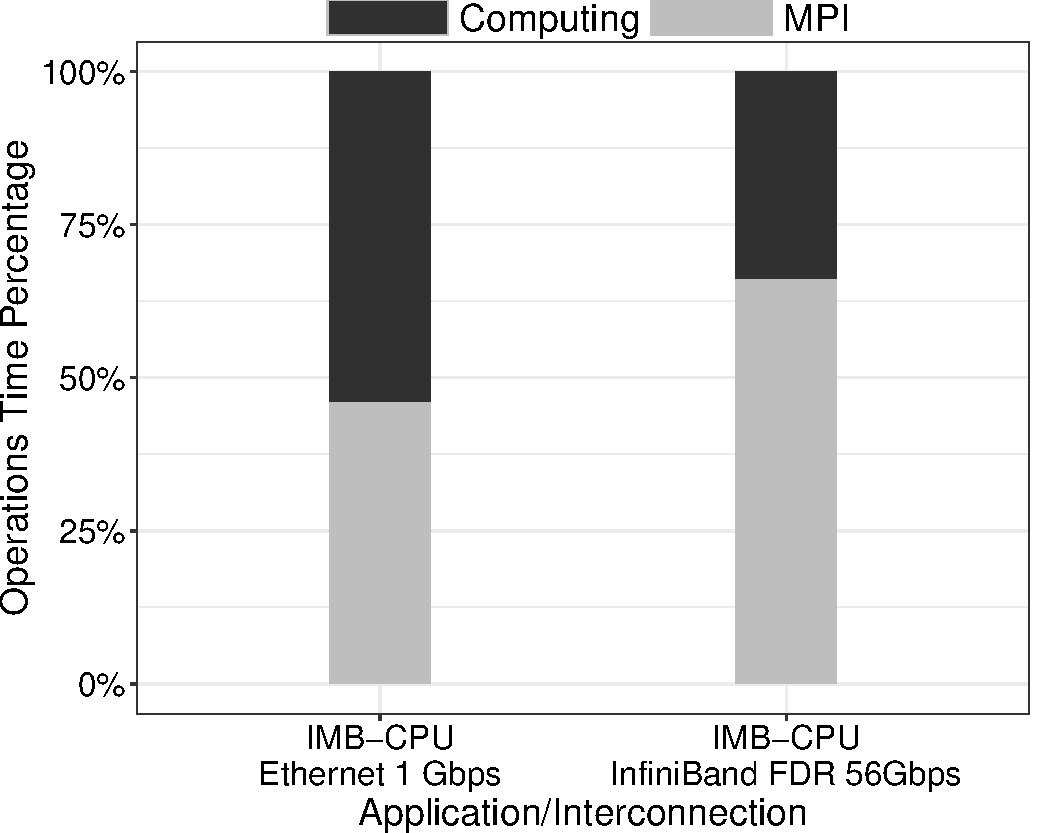
\includegraphics[width=0.38\textwidth]{SLIDES/img/IMB_CPU.percentage.pdf}
\end{figure}
Observations
\begin{itemize}
    \pause \item This app simulates the behavior of 8 levels of load unbalance, and this is evident in its tracing
    \pause \item As MPI\_Finalize spikes decrease, compute spikes increase.
    \pause \item MPI\_Init in IB increases the overall MPI time and percentage
    \pause \item CPU-Bound application with no gain in IB (similar to EP) 

\end{itemize}
\end{frame}

\begin{frame}{Conclusion}

Network interconnect performance remains a crucial aspect of HPC environments

\pause How do the communication characteristics of applications influence their performance?
\begin{itemize}
    \pause \item For applications with a high level of network dependency, it reaches or even exceeds the same level of importance as processing power
    \begin{itemize}
        \item FT $\approx$989\%
        \item IS $\approx$978\%
    \end{itemize} 
    \pause\item On the other hand, for applications that are CPU-Bound, a faster interconnection does not influence for improved performance
    \begin{itemize}
        \item EP 0\% gain or loss
        \item IMB-CPU less than 1\%
    \end{itemize}
\end{itemize}
\pause It is possible to optimize both performance and execution cost?
\begin{itemize}
    \pause\item YES!, BUT depends on the application characteristics, for example, FT have a huge gain in performance ($\approx$989\%) and also\\ optimized their cost $\approx$770\%
\end{itemize}
\end{frame}

\begin{frame}[t]{Future Work}
\begin{itemize}
    \item Perform the same assessment on leading public cloud providers (Amazon AWS, Google Cloud, and Microsoft Azure), considering all available network interconnects
   \begin{figure}
   
\includegraphics[width=0.3\textwidth]{SLIDES/logo/amazon.png}
   \hfill
   
\includegraphics[width=0.3\textwidth]{SLIDES/logo/Google_logo.png}
   \hfill
   
\includegraphics[width=0.3\textwidth]{SLIDES/logo/Azure_logo.png}
\end{figure}
    \pause\item Publish a paper using up-to-date instances price
\end{itemize}
\end{frame}
\logo{}

\begin{frame}{}
\begin{center}
\Huge{Thank you for your attention! Questions?}
\vfill
\Large{ammaliszewski@inf.ufrgs.br}
\vfill
\small{https://github.com/andermm/CMP223.git}
\end{center}
\end{frame}

\logo{
\includegraphics[width=1.3cm,keepaspectratio]{SLIDES/logo/ufrgs.png}~~~~~~~~~~~~~~~~~~~~~~~~~~~~~~~~~~~~~~~~~~~~~~~~~~~~~~~~~~~~~~~~~~~~~
%\hspace{\dimexpr\paperwidth-5cm-1pt}%
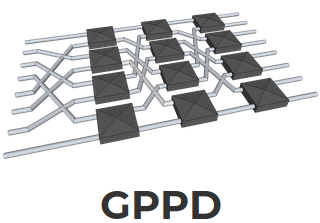
\includegraphics[width=1.3cm,keepaspectratio]{SLIDES/logo/GPPD-logo.png}~~~~~~~~~~~~~~~~~~~~~~~~~~~~~~~~~~~~~~~~~~~~~~~~~~~~~~~~~~~~~~~~~~~~~
%\hspace{\dimexpr\paperwidth-3cm-1pt}%

\includegraphics[width=1.5cm,keepaspectratio]{SLIDES/logo/inf-logo.png}%
}

\maketitle

\end{document}